\documentclass[12pt,xcolor=svgnames]{beamer}
% \documentclass[handout,xcolor=svgnames]{beamer} %Version imprimible
% -------------------------------------------------------------------
% Paquetes personalizados
% Definiciones de color:
% ============ == =====
\definecolor{azul}{rgb}{0.2,0.5,0.8}
\definecolor{azulcian}{rgb}{0.3,0.5,0.7}
\definecolor{azulleve}{rgb}{0.2, 0.4, 0.6}
\definecolor{beige}{rgb}{0.6,0.5,0.4}
\definecolor{burdeos}{rgb}{0.7,0.3,0.5}
\definecolor{burdeos2}{rgb}{.65,.12,.39}
\definecolor{gris}{rgb}{0.2,0.2,0.2}
\definecolor{gnome}{rgb}{0.55,0.3,0}
\definecolor{hierba}{rgb}{0.5,0.7,0.3}
\definecolor{marron}{rgb}{0.4,0.3,0.2}
\definecolor{morado}{rgb}{0.5,0.3,0.5}
\definecolor{naranja}{rgb}{1,.55,.25}
\definecolor{rojo}{rgb}{0.5,0,0}
\definecolor{rojo2}{rgb}{0.7,0,0}
\definecolor{verde}{rgb}{0.4,0.6,0.2}
\definecolor{verde2}{rgb}{0.2,0.5,0.2}
\definecolor{turquesa}{rgb}{0.3,0.7,0.5}
\definecolor{violeta}{rgb}{.5,0,.50}
\definecolor{vioscuro}{rgb}{.25,0,.40}

\usepackage{amsfonts}
\usepackage[spanish]{babel}
% Paquetes específicos de Beamer
\usepackage{beamerthemeshadow}
\usepackage[T1]{fontenc}
\usepackage{graphicx}
\usepackage{hyperref}
\usepackage[utf8]{inputenc}
%\usepackage{ragged2e} -> Justificado
\usepackage{tikz}
\usepackage{times}
\usepackage{listings}
\usepackage{colortbl}
\usetikzlibrary{arrows,shapes,snakes}

%---------Listing---------------------------------
%-- Formato de los listados de código
\lstset{ frame=Ltb,
     framerule=0pt,
     boxpos=c,
     aboveskip=0.5cm,
     framextopmargin=3pt,
     framexbottommargin=3pt,
     framexleftmargin=0.4cm,
     framexrightmargin=-3cm,
     framesep=0pt,
     rulesep=.4pt,
     %
     stringstyle=\ttfamily\color{burdeos},
     identifierstyle=,
     showstringspaces = false,
     basicstyle=\small\ttfamily,
     commentstyle=\color{violeta},
     keywordstyle=\bfseries,
   }

% minimizar fragmentado de listados
\lstnewenvironment{listing}[1][]
   {\lstset{#1}\pagebreak[0]}{\pagebreak[0]}

% estilo de consola
\lstdefinestyle{consola}
   {basicstyle=\scriptsize\bf\ttfamily,
    backgroundcolor=\color{gray75},
   }

\lstdefinestyle{consola-trans}
   {basicstyle=\scriptsize\bf\ttfamily,
   }

%estilo para C
\lstdefinestyle{C}
   {language=C,
     %
     numbers=left,
     numbersep=15pt,
     numberstyle=\tiny,
     numberfirstline = false,
     breaklines=true,
     emptylines=2,
   }

%estilo para C++
\lstdefinestyle{C++}
   {language=C++,
     %
     breaklines=true,
     emptylines=2,
   }

%estilo para Haskell
\lstdefinestyle{haskell}
   {language=Haskell,
     %
     breaklines=true,
     emptylines=2,
   }

\mode<presentation>
{
\usefonttheme{structuresmallcapsserif}
%\useoutertheme{shadow}
% -------------------------------------------------------------------
% Elección del tema Beamer
% -------------------------------------------------------------------
% Más llamativos:
% === ==========
%\usetheme{Copenhagen}
%\usetheme{Darmstadt}
%\usetheme{Frankfurt}
%\usetheme{Ilmenau}
%\usetheme{Szeged}
%\usetheme{Warsaw}
% -------------------------------------------------------------------
% Menos llamativos:
% ===== ==========
%\usetheme{Antibes}
%\usetheme{Bergen}
%\usetheme{Berkeley}
%\usetheme{Berlin}
%\usetheme{boxes}
\usetheme{CambridgeUS}
%\usetheme{Dresden}
%\usetheme{Goettingen}
%\usetheme{Hannover}
%\usetheme{Madrid}
%\usetheme{Malmoe}
%\usetheme{Marburg}
%\usetheme{Montpellier}
%\usetheme{PaloAlto}
%\usetheme{Pittsburgh}
%\usetheme{Rochester}
%\usetheme[height=7mm]{Singapore}
% --------------------------------------------------------------------
%%\useinnertheme{rounded}
%%\setbeamercovered{transparent}
}
% --------------------------------------------------------------------
% Esquema de color:
% ======= == =====
%\usecolortheme{albatross}
%\usecolortheme{default}
%\usecolortheme{beetle}
%\usecolortheme{crane}
%\usecolortheme{dove}
%\usecolortheme{fly}
%\usecolortheme{lily} % SOI/SOII
%\usecolortheme{orchid}
%\usecolortheme{rose}
%\usecolortheme{seahorse}
%\usecolortheme{seagull}
%\usecolortheme{sidebartab}
%\usecolortheme{wolverine}
%\usecolortheme[named=yellow]{structure}
%\usecolortheme[named=purple]{structure}
%\usecolortheme[named=blue]{structure}
%\usecolortheme[named=rojo]{structure}
%\usecolortheme[named=gnome]{structure}
\usecolortheme[named=rojo]{structure}
% --------------------------------------------------------------------
%\hypersetup{colorlinks=true,%
%    linkcolor=rojo2,%
%    citecolor=rojo,%
%    filecolor=rojo,%
%    menucolor=rojo,%
%    pagecolor=rojo,%
%    urlcolor=rojo}
% --------------------------------------------------------------------
% Color del tema:
% ===== === ====
%\usecolortheme[named=DarkBlue]{structure}
% --------------------------------------------------------------------
% Modificación del fondo
%\usepackage{fondo}
% --------------------------------------------------------------------
% Definición de comportamiento en cada nueva subsección:
%  -> Título en función de sección y subsección
\AtBeginSection[]
{
  \begin{frame}<beamer>
   \frametitle{Table of contents}
   \transdissolve
   \tableofcontents[currentsection,currentsubsection]
  \end{frame}
}
\AtBeginSubsection[]
{
  \begin{frame}<beamer>
   \frametitle{Table of contents}
   \transdissolve
   \tableofcontents[currentsection,currentsubsection]
  \end{frame}
}
% --------------------------------------------------------------------
% Márgenes laterales (adecuación con el fondo)
%%\setbeamersize{text margin left=1.2cm, text margin right=1.2cm}
% Cambiar márgenes
\newenvironment{cambiarmargen}[2]{%
 \begin{list}{}{%
  \setlength{\topsep}{0pt}%
  \setlength{\leftmargin}{#1}%
  \setlength{\rightmargin}{#2}%
  \setlength{\listparindent}{\parindent}%
  \setlength{\itemindent}{\parindent}%
		  \setlength{\parsep}{\parskip}%
		  }%
 \item[]}{\end{list}}
% --------------------------------------------------------------------n

% Info
% ====
\title[FreeAlgView]{FreeAlgView}
\author[Aarón Bueno]{Aarón Bueno Villares\\$<$abv150ci@gmail.com$>$}
\institute[UCA \& FHWS]{\textit{Universidad de Cádiz} \\ \textit{Hochschule für
    angewandte Wissenchaften Würzburg-Scheweinfurt}}
\subject{Final degree project}
\date{December 2012}
% -------------------------------------------------------------------
% Directorio de imágenes
\graphicspath{{./images/}}
% -------------------------------------------------------------------
% \setbeamersize{text margin left=1.6em,text margin right=1.6em}

% Comienza el documento
\begin{document}
% Tikz -> Imágenes
\tikzstyle{every picture}+=[remember picture]
% Entorno matemático
\everymath{\displaystyle}

\begin{frame}
  \titlepage
\end{frame}

\begin{frame}{Table of contents}
  \transdissolve
  \tableofcontents
\end{frame}

\section{The project}

\begin{frame}{Definition}
  \begin{block}{Definition}
    \begin{center}
      \textit{A libre and learning-oriented algorithm animation application}
    \end{center}
  \end{block}

  \pause

  \begin{block}{Purpose}
    \begin{enumerate}
    \item Make easier to understand algorithms by means of animations.
    \item Not only for teachers, also for students:
      \begin{center}
        \textit{Teaching $\neq$ Learning}
      \end{center}
    \item Custom animations for any custom algorithm.
    \end{enumerate}
  \end{block}
\end{frame}

\section{State of art}

\begin{frame}{Old systems}
  \begin{block}{Features}
    \begin{itemize}
    \item Calls to graphic primitives inside an algorithm.
    \item Animations for any algorithm.
    \end{itemize}
  \end{block}

  \begin{block}{Disadvantages}
    \begin{itemize}
    \item Graphic calls spoils
q the textual algorithm.
    \item Non-modifiable animations.
    \end{itemize}
  \end{block}
\end{frame}

\begin{frame}{New systems}
  \begin{block}{Features}
    \begin{itemize}
      \item Prebuilt animations.
      \item \url{http://algoviz.org}
    \end{itemize}
  \end{block}

  \begin{block}{Disadvantages}
    \begin{center}
      \textit{Inflexibility}: only you can use the application offers you, and
      no more.
    \end{center}
  \end{block}
\end{frame}

\begin{frame}{Preliminary planned features}

  \begin{block}{Independence algorithm/animation}
    \begin{itemize}
    \item Language for describing algorithms.
    \item Language for describing animation.
    \end{itemize}
  \end{block}

  \begin{block}{User participation}
    \begin{itemize}
    \item Control step by step.
    \item Perhaps, a terminal to write ``graphical'' commands.
    \end{itemize}
  \end{block}

\end{frame}

\section{FreeAlgView in action}

\begin{frame}{FreeAlgView in action}
  \begin{block}{FreeAlgView}
    \textit{A little demonstration}
  \end{block}

  \pause

  \begin{block}{Additional information}
    \url{http://freealgview.blogspot.com}
  \end{block}
\end{frame}

\section{Technical issues}

\begin{frame}{Backgrounds}

  \begin{block}{Properties}
    \begin{itemize}
    \item C++11.
    \item GPL v3.
    \item Multiplataform.
    \end{itemize}
  \end{block}

  \begin{block}{Libraries}
    \begin{itemize}
    \item Qt4.
    \item QPainter.
    \end{itemize}
  \end{block}

  \begin{block}{Tools}
    \begin{itemize}
    \item CMake.
    \item Bisonc++/Flexc++
    \end{itemize}
  \end{block}

\end{frame}

\begin{frame}{Design}
  \begin{center}
    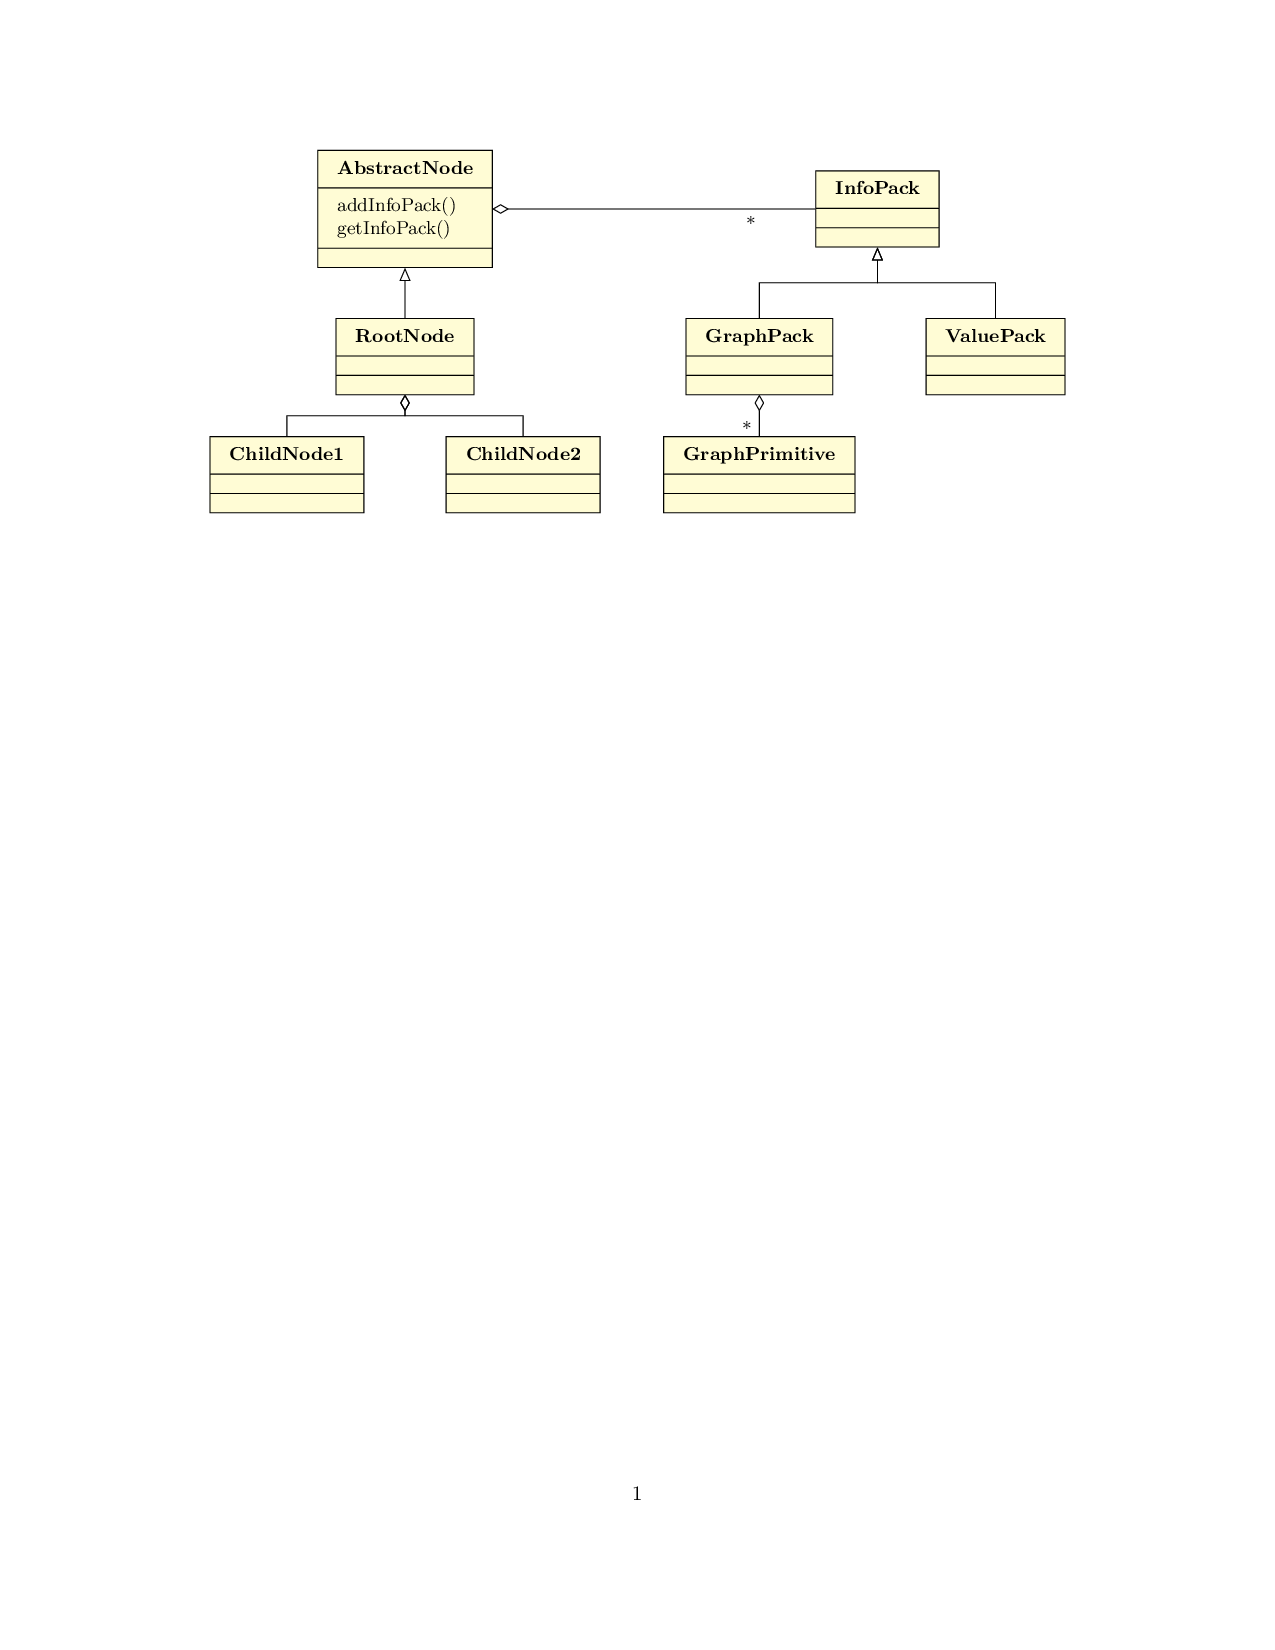
\includegraphics[scale=0.25]{class-diagram.png}
  \end{center}
\end{frame}

\section{End of presentation}

\begin{frame}{Questions}
  \begin{block}{}
    \begin{center}
      \textbf{\Large{Thank You very much!}}
    \end{center}
  \end{block}

  \begin{block}{}
    \begin{center}
      \textbf{\Large{Any questions?}}
    \end{center}
  \end{block}
\end{frame}

\end{document}
